\everymath{\displaystyle}
\documentclass{beamer}
% \documentclass[handout]{beamer}

%\usepackage[pdftex]{color,graphicx}
\usepackage{amsmath,amssymb,amsfonts}

\mode<presentation>
{
  % \usetheme{Darmstadt}
  % \usetheme[hideothersubsections]{Hannover}
  % \usetheme[hideothersubsections]{Goettingen}
  \usetheme[hideothersubsections, right]{Berkeley}

  \usecolortheme{seahorse}
  % \usecolortheme{dolphin}
  \usecolortheme{rose}
  % \usecolortheme{orchid}

  \useinnertheme[shadow]{rounded}

  \setbeamercovered{transparent}
  % or whatever (possibly just delete it)
}

\mode<handout>{
  \setbeamercolor{background canvas}{bg=black!5}
  \usepackage{pgfpages}
  \pgfpagesuselayout{4 on 1}[a4paper,border shrink=5mm, landscape]
}

\usepackage[brazilian]{babel}
% or whatever

% \usepackage[latin1]{inputenc}
\usepackage[utf8]{inputenc}
% or whatever

\usepackage{times}
%\usepackage[T1]{fontenc}
% Or whatever. Note that the encoding and the font should match. If T1
% does not look nice, try deleting the line with the fontenc.


\title%[] % (optional, use only with long paper titles)
{Distribuições de Probabilidades}

\subtitle
{Distribuições de Probabilidades Discretas} % (optional)

\author%[] % (optional, use only with lots of authors)
{Felipe Figueiredo}% \and S.~Another\inst{2}}
% - Use the \inst{?} command only if the authors have different
%   affiliation.

\institute[UNIAN] % (optional, but mostly needed)
{Centro Universitário Anhanguera de Niterói}
  % \inst{1}%
  % Department of Computer Science\\
  % University of Somewhere
  % \and
  % \inst{2}%
  % Department of Theoretical Philosophy\\
  % University of Elsewhere}
% - Use the \inst command only if there are several affiliations.
% - Keep it simple, no one is interested in your street address.

\date%[] % (optional)
{}

% \subject{Talks}
% This is only inserted into the PDF information catalog. Can be left
% out. 



% If you have a file called "university-logo-filename.xxx", where xxx
% is a graphic format that can be processed by latex or pdflatex,
% resp., then you can add a logo as follows:

\pgfdeclareimage[height=1.6cm]{university-logo}{../logo}
\logo{\pgfuseimage{university-logo}}



% Delete this, if you do not want the table of contents to pop up at
% the beginning of each subsection:
\AtBeginSubsection[]
%\AtBeginSection[]
{
  \begin{frame}<beamer>{Sumário}
    \tableofcontents[currentsection,currentsubsection]
  \end{frame}
}


% If you wish to uncover everything in a step-wise fashion, uncomment
% the following command: 

\beamerdefaultoverlayspecification{<+->}


\begin{document}

\begin{frame}
  \titlepage
\end{frame}

\begin{frame}{Sumário}
  \tableofcontents
  % You might wish to add the option [pausesections]
\end{frame}


%% Template
% \section{}

% \subsection{}

% \begin{frame}{}
%   \begin{itemize}
%   \item 
%   \end{itemize}
% \end{frame}

% \begin{frame}
%   \begin{columns}
%     \begin{column}{5cm}
%     \end{column}
%     \begin{column}{5cm}
%     \end{column}
%   \end{columns}
% \end{frame}

% \begin{frame}{}
%   \includegraphics[height=0.4\textheight]{file1}
%   \includegraphics[height=0.4\textheight]{file2}
%   \includegraphics[height=0.4\textheight]{file3}
%   \begin{figure}
%     \caption{}
%   \end{figure}
% \end{frame}

\section{Variáveis Aleatórias}

\subsection{Tipos de Variáveis}
\begin{frame}{Variáveis Aleatórias}
\begin{definition}
  % Valor numérico associado a um experimento aleatório
  Uma \alert{variável aleatória} é uma variável (tipicamente
  representada por $x$) que tem um único valor numérico associada a um
  experimento aleatório
\end{definition}
\begin{itemize}
\item Discretas% (quantidade contável de valores)
\item Contínuas% (escala contínua de valores)
\end{itemize}
\end{frame}

\subsection{Variáveis Discretas}
\begin{frame}{Variáveis Discretas}
  \begin{definition}
    Uma variável aleatória \alert{discreta} pode assumir uma
    quantidade contável de valores
  \end{definition}
  \begin{example}
    \begin{itemize}
    \item Número de filhos em uma família
    \item Quantidade de pacientes em um dia no consultório
    \end{itemize}
  \end{example}
\end{frame}

\begin{frame}{Representação em tabela}
  \begin{example}
    Seja x o número de filhos em uma família. 

    \begin{tabular}{c|ccccc}
      x & 0 & 1 & 2 & 3 & 4\\
      \hline
      P(x) & 0.15 & 0.30  & 0.40 & 0.10 & 0.05\\
    \end{tabular}

    O valor esperado $E[x]$ (de filhos por família) é:
    \begin{displaymath}
      \sum x P(x) = 0 \times 0.15 + 1 \times 0.30 + 2 \times 0.40
      \ldots = 1.6
    \end{displaymath}
  \end{example}
\end{frame}

\begin{frame}{Representação gráfica}
  \begin{figure}
    \centering
    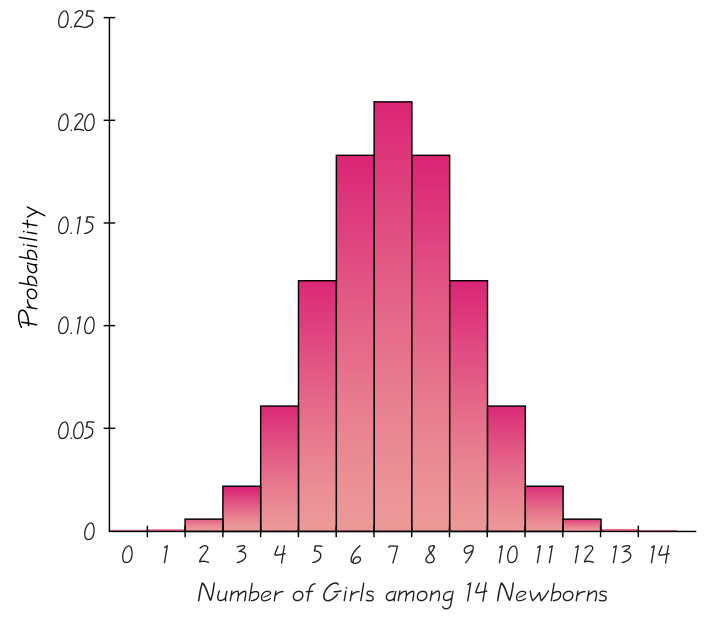
\includegraphics[height=0.6\textheight]{Prob_II/discreta}
    \caption{A distribuição de uma variável discreta (Fonte: Triola,
      2004}
  \end{figure}
\end{frame}

\subsection{Variáveis Contínuas}
\begin{frame}{Variáveis Contínuas}
  \begin{definition}
    Uma variável aleatória \alert{contínua} pode ser associada a
    medições em uma escala contínua (e infinita) de valores
  \end{definition}
  \begin{example}
    \begin{itemize}
    \item Quantidade de leite produzido por uma vaca em um dia
    \item Expectativa de vida de um paciente terminal
    \end{itemize}    
  \end{example}
\end{frame}

% \begin{frame}{Representação gráfica}

%   \begin{itemize}
%   \item 
%   \end{itemize}
% \end{frame}

\section{Distribuições de Probabilidade}
\begin{frame}{Distribuições de Probabilidade}
  \begin{definition}
    Uma \alert{distribuição de probabilidade} é um gráfico, tabela ou
    fórmula que relaciona a cada valor que a variável aleatória pode
    assumir a sua probabilidade
  \end{definition}
  Os pré-requisitos para uma função ser uma Função de Probabilidade
  são:
  \begin{itemize}
  \item $\sum P(x) = 1$, onde $x$ percorre todos os valores possíveis
  \item $0 \le P(x) \le 1$, para todo $x$
  \end{itemize}
\end{frame}

\subsection{Distribuições Discretas}

% \subsection{Bernoulli}
\begin{frame}{A distribuição de Bernoulli}
  \begin{itemize}
  \item Um ensaio de Bernoulli é teste com desfecho 0 ou 1 (negativo
    ou positivo)
  \item Probabilidade de sucesso $p$
  \item Probabilidade de fracasso $1-p$
  \item Notação: $X \sim Bern(p)$
  \item Valor esperado: $E[x] = p$
  \end{itemize}
\end{frame}

% \subsection{Binomial}
\begin{frame}{A distribuição Binomial}
  \begin{definition}
    Um \alert{experimento binomial} é um experimento de probabilidade que possui as seguintes propriedades:

    \begin{itemize}
    \item O experimento é repetido por um $n$ fixo de tentativas independentes
    \item Há apenas 2 resultados possíveis em cada tentativa (sucesso e fracasso)
    \item A probabilidade de sucesso $P(S)$ é a mesma em todas as tentativas
    \item A variável aleatória $x$ contabiliza o número de sucessos do experimento.
    \end{itemize}
  \end{definition}

Fonte: Larson \& Farber, 2010.
\end{frame}

\begin{frame}{A distribuição Binomial}
  \begin{itemize}
  \item Quando executamos $n$ ensaios de Bernoulli
    \alert{independentes}, encontramos a distribuição Binomial
  \item Com $n$ ensaios (cada um com prob. $p$), temos a contagem $x$
    de sucessos (desfecho = 1)
  \item Notação $X \sim Bin(n,p)$
  \item Valor esperado: $E[x]=np$
  \end{itemize}
\end{frame}

\begin{frame}{A distribuição Binomial}
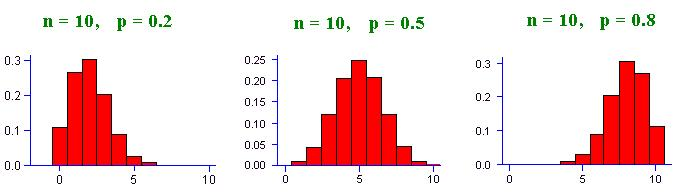
\includegraphics[width=\textwidth]{Prob_II/binomial}
\end{frame}

\begin{frame}{Aumentando o tamanho da amostra}
  \begin{itemize}
  \item Quanto maior o tamanho $n$ da amostra, mais ``suave'' a
    distribuição binomial, e mais simétrica
  \item O histograma vai ficando cada vez mais parecido com uma curva
  % \item https://www.youtube.com/watch?v=6YDHBFVIvIs (Galton board)
  % \item https://www.youtube.com/watch?v=9xUBhhM4vbM (Galton machine)
  \end{itemize}
  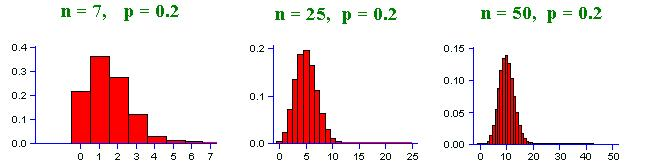
\includegraphics[width=\textwidth]{Prob_II/binomial2}

\end{frame}

\begin{frame}{Aumentando o tamanho da amostra}
  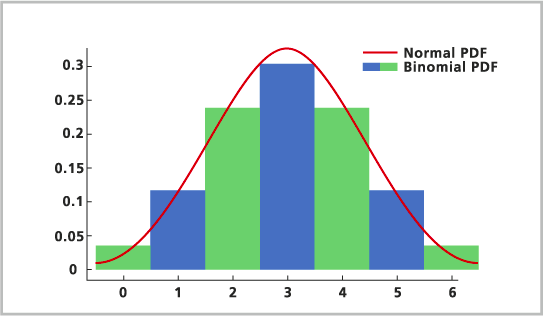
\includegraphics[width=\textwidth]{Prob_II/aproximacao}

  (Vídeos: Galton board e Galton machine)
\end{frame}

\end{document}
